\documentclass[12pt, letterpaper]{article}
 
\usepackage{amssymb,amsmath}
\usepackage{fancyvrb}
\usepackage{xcolor}
\usepackage[margin=2cm]{geometry}
\usepackage{array}        
\usepackage{pifont}
\usepackage{titlesec}
\usepackage{graphicx}
 
\setlength{\headheight}{18pt}
\titleformat*{\section}{\large\bfseries}

\usepackage[pdftitle={COMP3106 Assignment 3},
            pdfsubject={Carleton University, 
                        COMP3106, Fall 2021},
            pdfauthor={Jersey Aubin-Déry}]
            {hyperref}

\usepackage{lastpage}

\usepackage{fancyhdr}
\pagestyle{fancy}
\fancyhf{} % sets both header and footer to nothing
\renewcommand{\headrulewidth}{0pt}
\lfoot{}
\cfoot{}
\rfoot{\the\numexpr\thepage-1 \text{ of 6}}

\setlength\parindent{0pt}

\author{Eric Pham: 101104095\\Jersey Aubin-Déry: 101079607}
\date{December 10, 2021}
\title{Chess AI With Iterative-Depth Minimax\vspace{15em}}

% --------------------------------------------------------------------------- %   
\begin{document}

\maketitle
\thispagestyle{empty}
\clearpage

\textbf{Statement of Contributions}

\medskip

Group members made significant contributions and approximately equal contributions each.
\medskip

\begin{tabular}{m{8cm} m{8cm}}
  Jersey & Eric \\
  \begin{itemize}
    \item Came up with project ideas
    \item Improved AI implementation
    \item Chess game implementation
    \item Report and typeset the report
    \item Validation
  \end{itemize} & 
  \begin{itemize}
    \item AI implementation
    \item Portions of chess game implementation and game logic
    \item Report
  \end{itemize}
  

\end{tabular}

\textbf{Introduction}

\medskip

Early on in class, we learned about the minimax algorithm, which was especially useful for
multiplayer turn-based games where each player tries to play optimally, against the other
players. So it seemed fitting to apply this knowledge to the game known as chess. For
performance reasons, it also seemed like a good application of the alpha-beta pruning algorithm.
Using an AI following these methods, we can create an interactive chess game that only requires
one player, who would play against this AI.

\medskip

There were a few other details before implementing the AI. As there are many pieces and positions
on a chess board, there are many different possible moves a player can make in any given turn,
so we wanted to implement the minimax algorithm at a fixed depth, and utilize heuristic values
in the leaf nodes to estimate the optimal move without too much delay.

\medskip

For the implementation, we decided on creating an interactive CLI program for the chess game made
in Python. The agent is a model-based agent, where the chess board and pieces are modeled using
Python classes and a 2D list. This environment model is also useful for displaying and keeping track of
the game progress.

\bigskip

The environment details are as follows:

\medskip

For a performance measure, some kind of game board score can be used. Things to take into account
for the score are the number of pieces in the board state, which chessman they are, the configuration
of these pieces, and the number of possible actions available to the agent. An overall performance
score would be the difference between an agent's score and the adversary's score, as it would also
let the agent know if it is more likely to win or not with that specific board state. This score can
be used for estimating heuristic values of possible future states as well. The environment itself
would be the board and pieces on the board. The actuators can be “actions” or “moves”, which is when an
agent takes a piece from the board and moves it to a different valid location on the board, based on
the game rules. The sensors would then be the board state. These can be provided by a model of the board
with a simple API.

\clearpage

The properties of the environment are:
\begin{itemize}
  \item Fully observable: agent has complete access to the game/board state
  \item Multiple agent: The AI and the adversary are agents in the game
  \item Deterministic: The next state (pieces and board state), only depends
  on the currentstate and actions
  \item Sequential: The way an agent plays will definitely affect what possible
  moves will be available in the future
  \item Semi-dynamic: If the timer is considered to be part of the environment,
  then it will change while the agent “thinks”, and needs to be taken into account
  for its next action
  \item Discrete: The state is discrete (from a set number of pieces and squares
  on a board), time is discrete as it is only considered in seconds, and precepts
  and actions are discrete for the same reasons the state is
  \item Known: Every action/move has a specific outcome that the agent will always know
\end{itemize}

\medskip

To conclude, this project sets out to solve the following problem: can we use an AI to
efficiently take the role of a player in a game of chess?

\bigskip

\textbf{Methods}

The implementation was created in Python. Below are the implementation details:

\medskip

\underline{The AI}

\medskip

The AI uses minimax and alpha-beta pruning to find the optimal move. It does so for a fixed-depth,
and the leaf nodes return an estimated value (a heuristic) of the game board state/heuristic instead
of terminal values, unless it reaches a terminal state.

\medskip

For the most part, the implementation of minimax and alpha-beta pruning was based off of the pseudocode
given from in-class. However, the one notable change is that the terminal state includes when the
AI's timer has run out in addition to when the game is finished, when the constant minimax depth has been exceeded.

\medskip

The algorithm is implemented as a separate portion from the main program, with a simple callable function
called startMininmax(), which requires a game board to know the starting state, the AI player's colour to know
which player to compute the maximum value for, and a time limit to make sure the algorithm does not take too much
of the player's time. In the main program when it is the AI player's turn, startMininmax() can be called to
find the optimal move, and request it in the game board as the AI's chosen move.

\medskip

In startMininmax(), the minimax algorithm may be run several times, depending on the time limit given.
The first run will be at a depth of 1, and if there is time left, it will run again at an incremented depth.
Eventually, the time will run out and the optimal action chosen from the previous run will be returned.
This timing algorithm attempts to maximize the depth of the minimax search which would make the returned
optimal action more accurate, all without exceeding the given time limit.

\clearpage

\underline{The Heuristic}

\medskip

The game board implementation includes the gameScore() function that returns an estimated value of the
board's state. As explained earlier, this value is determined using the caller player's score
(which for the AI, is the AI player), subtracted by the adversary's score. And each player's score is
determined by the amount of pieces they have on the board, which kinds of pieces they have on the board,
and the number of possible actions they can take with them. The values of the piece types are
multiplicative to the number of pieces that there are, which is added to the overall score.

\medskip

While the weighting of each piece can be changed, what's important is that the weighting in order of highest to lowest is:

\begin{center}
  king $\gg$ queen $>$ rook $>$ bishop $\approx$ knight $>$ pawn
\end{center}

\medskip

The number of valid actions is also assigned a value, which is less than all the pieces.
At the end, the number of valid actions times its weight can be added to the player's score too.

\medskip

This heuristic is based on Claude Shannon's evaluation function formulated in 1949.

\medskip

\underline{Disadvantages}

\medskip

With a limited depth, our heuristic tends to reward capturing pieces too much. This causes more stalemates.
Without taking into account configuration of pieces, the heuristic will value useless pieces/pawns as much as useful pieces.
The minimax method assumes that the player is playing “optimally”. In this case, “optimally” is in accordance
with the heuristic, which means the algorithm assumes that the player is attempting to capture pieces more in
the short term as well.

\medskip

\underline{Validation}

\medskip

As chess is unsolved, there is no way to know if the AI is correct unless it wins in a field test.
To do so, as the AI can accept input from the user or another command line program, one can hook up a
chess engine as one of the players. As a proof of concept, we first played it against one of the AI
opponents on chess.com with an elo of around 1000, which would be slightly above a casual chess player.
In doing so, it was able to beat the opponent when our AI had a 10 second period to think. However,
against a 1300 rated player, the AI was starting to struggle with making moves that looked far enough
into the future. This shows that the AI is able to at least make moves that lead to a future game board
that appears to be in its favour, as well as the heuristic correctly gauging whether or not the current
game board is good for the AI or not.

\clearpage

\textbf{Results}

\medskip

At the end of this project, we have a working chess implementation where a user can play against the AI.
The AI takes its own time to decide its next move whenever it is its turn, and it tends to choose moves
that will guide it to capturing the user's pieces. 

\medskip

\underline{Positive results}:

\medskip

The implementation works, and it does not take too much time to work. The AI is also fairly flexible with
the heuristic by being able to adjust the chessmen weights, and with the time limit. A trade off can be
found between the time it takes the AI to compute its optimal action and the accuracy of the minimax
algorithm with the fixed-depth which is affected by the time limit.

\medskip

With its abilities, it was able to beat an opposing AI with a rating of 1000, although our AI did take
substantially longer in order to perform its actions.

\begin{figure}[htb]
  \centering
  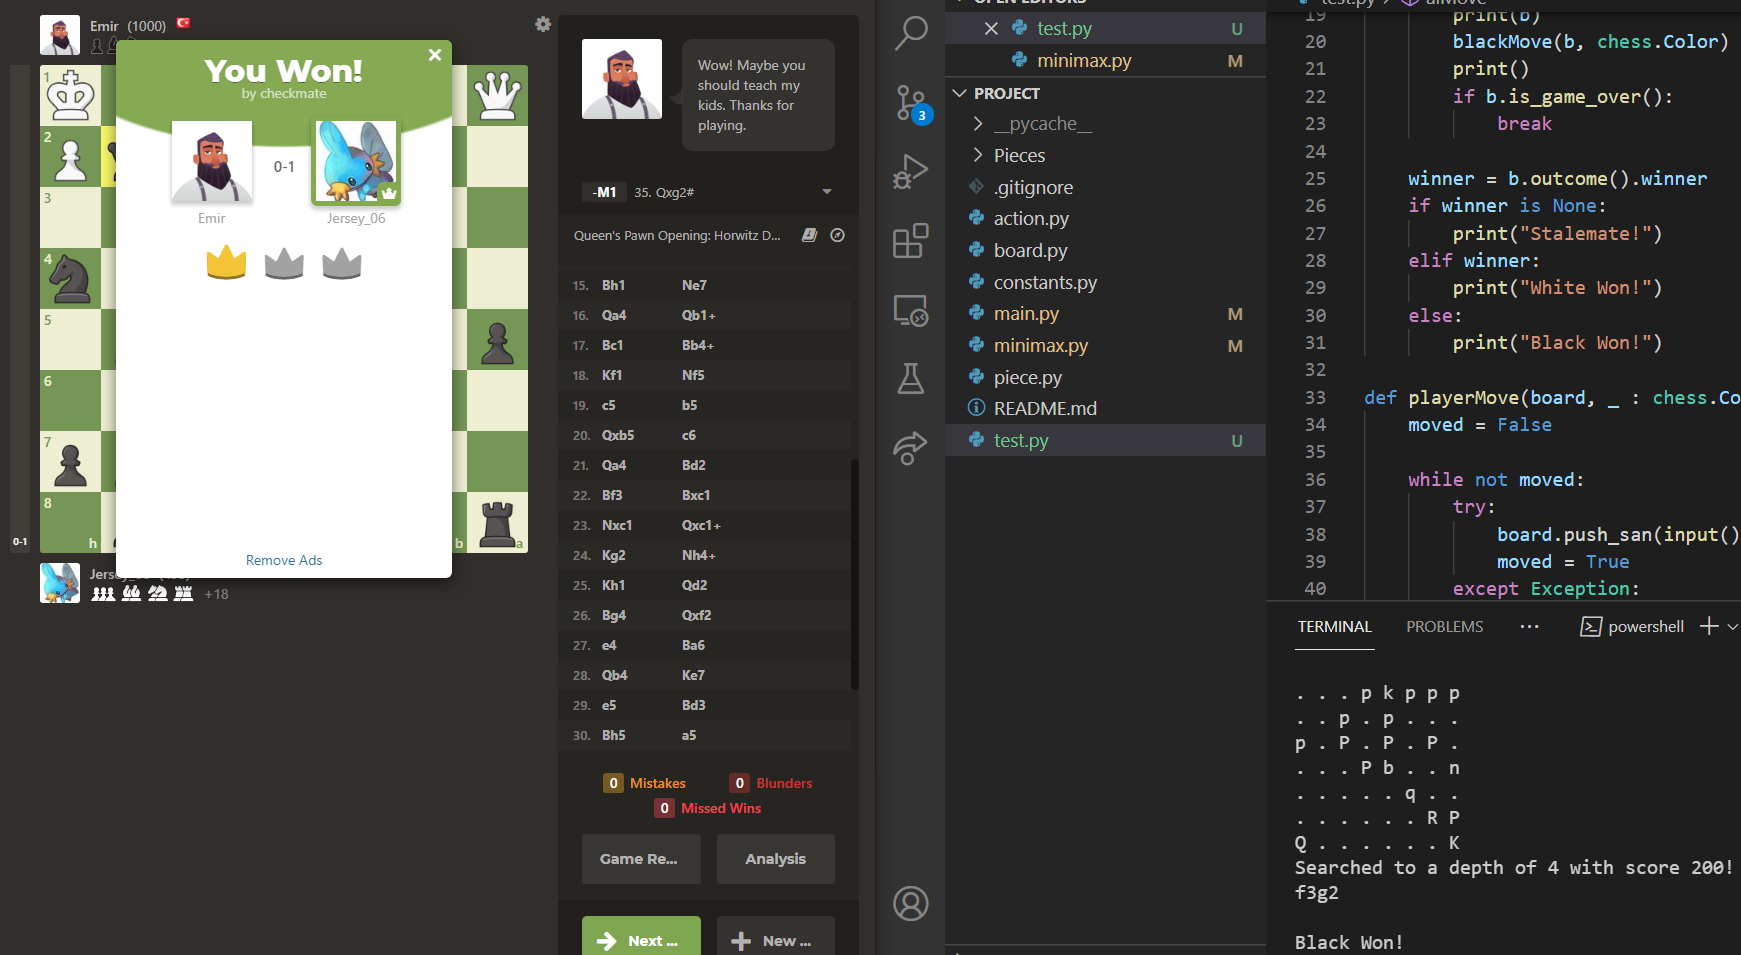
\includegraphics[width=\linewidth]{Figure_1.png}
  \caption{The AI beating a 1000 rated opponent.}
  \label{fig:ai1}
\end{figure}

\medskip

\underline{Negative results}:

\medskip

As the AI values movement and capture of pieces on top of not having much future vision, the AI will
sometimes blunder \footnote{Make a move that loses a piece} because of its short sighted vision.
The AI will also choose the first move it evaluates whenever it encounters multiple moves with the
same expected value, which will lead the AI to repeat moves if the opponent cannot make a proper attack.
This effectively wastes the AI's turns and will allow the opponent to potentially move into an advantageous
position while the AI does nothing of any value.

\clearpage

\textbf{Discussion}

\medskip

Using the minimax algorithm, the AI is able to act as a chess player in the sense that it can choose
desirable moves within a reasonable amount of time.

\medskip

\underline{Limitations}:

\medskip

One of the biggest limitations of the project are computing power and the AI's time limit, as the
minimax algorithm can be heavy on those factors. Much of the project attempts to workaround these two
factors. This includes the addition of alpha-beta pruning, stopping at a fixed-depth, using a heuristic
value to estimate terminal states, and the per-AI turn timer.

\medskip

As the AI is only able to search to a depth of 5 on average, it is unable to plan far enough into the
future. For example, moving a pawn forwards does not change much about the current state of the board,
so it is unable to see that moving the pawn to the other side of the board will allow it to promote the
piece and have a higher score. This also means that a checkmate in a few moves might not be seen as it
did not have enough time to find it.

\medskip

Another limitation is the fact that the AI's heuristic is mainly considering the pieces on the board.
This coupled with its relatively short future vision leads the AI to making short term reward goals
that might be detrimental to it in the long run. For example, the AI might capture a piece because it
can, not looking at the consequences of capturing that piece.

\medskip

Finally, because the AI looks at moves in order and the heuristic is deterministic, the AI will always
perform the same action when given multiple equally valued actions. This could have been remedied by
adding some negligible non-zero random value to the heuristic which would not change an ideal move,
but would allow for the AI to select from any equally tied moves, or if the AI would look at all
valid moves in a random order.

\medskip

\underline{Future work}:

\medskip

Something that was missed in our heuristic implementation was taking into account the configuration of pieces.
Certain configurations, such as having the bishop ``pair'' or having a large center should be able to increase
the value of a player's score, while configurations such as blocked or isolated pawns can be valued less than
the rest of the pawns. These changes to the heuristic could increase the AI's strategy when finding the optimal
move in minimax.

\medskip

We can also make use of different heuristics with their own strategies and advantages to tackle different portions
of a chess game. For example, a specific heuristic can be used with the endgame to better estimate optimal moves
for an endgame. In the endgame, pawns become vastly more powerful as they are able to be promoted into pieces
such as a queen. Also, as chess has been solved for six pieces, one could incorporate the tablebase into the AI.
This would result in a much larger program size, however it comes with the tradeoff of a much faster computation
of moves as well as perfect accuracy. On the other hand, openings have also been studied in chess to such a degree
that high end play relies on openings in order to have a known good position. This would result in both faster and
more accurate moves at the beginning.

\medskip

There is also a trade off of the time the AI can make moves throughout a game that has yet to be accounted for.
There are several strategies that can be used to deal with this. For example, the timer can be strategically
changed throughout the game. If the AI is running out of time, it would have to try and search for less time
in order to not get flagged\footnote{Ending a game due to time}.

\medskip

Finally, as many possible chess positions are reachable from different move orderings, implementing a
cache would help speedup the AI. For example, moving the \textit{d} pawn, the opponent's \textit{d} pawn,
then the \textit{e} pawn would result in the same position as moving the \textit{e} pawn, the opponent's
\textit{d} pawn, and then the \textit{d} pawn. Currently, the AI will search through both of these trees
which would result in the same value while wasting time, whereas caching would allow the AI to see it has
already visited a board position and use the previously found value, potentially saving having to search a
couple to dozens of moves in the future if it had more power. This would allow it to also find new board
positions. Also, the time saved through caching can be used to search with further depth for a more accurate
optimal move, or saved for later in the game if the AI needs it.

\bigskip
\bigskip
\bigskip

\textbf{Sources}

\medskip

Holden, Matthew. ``Alpha-Beta Pruning.'' COMP 3106: Intro to AI, 29 Sep. 2021, Carleton University, Ottawa. Lecture.

\medskip

Shannon, Claude. ``Programming a Computer for Playing Chess.'' Bell Telephone Laboratories, 
Inc., 8 Nov.1949, Murray Hill, N.J.


% --------------------------------------------------------------------------- %   
\end{document}
% --------------------------------------------------------------------------- %   